%%%%%%%%%%%%%%%%%%%%%%%%%%%%%%%%%%%%%%%%%%%%
% 
% Last edits: Nov 9, 2016
%%%%%%%%%%%%%%%%%%%%%%%%%%%%%%%%%%%%%%%%%%%%

\documentclass[12pt]{article}
\usepackage{natbib}
\usepackage[letterpaper, margin=1.1in]{geometry}
\usepackage{graphicx}
\usepackage{wrapfig}
\usepackage{enumitem}
\setlist[enumerate]{itemsep=0mm}
\usepackage{multirow}
\usepackage{lscape}
\usepackage{caption}
\usepackage{subcaption}
\usepackage{hyperref}

\begin{document}
\noindent{Alexandra Pulwicki \\ \today}

\begin{center}
\Large \textbf{Results\\ Observations}
\end{center}

- correlation matrix between topo params (sampled and full)

\section*{Overview}
This is a document that shows the sampled and full ranges of topographic parameters and then goes into the multiple linear regression and Bayesian model averaging that was used to explain SWE with topographic parameters. 


\pagebreak

%%%%
\section{Topographic parameters of study sites}
%%%%

One method of interpolating snow water equivalent (SWE) is to relate the observed SWE with topographic parameters derived from a digital elevation model (DEM) of the study area. The imagery we were using was from the SPOT-5 DEMs and were provided at no cost by the French Space Agency (CNES) through the SPIRIT International Polar Year project \citep{Korona2009}. The DEM has a cell size fo 40x40 m. The following topographic parameters were calculated from the DEM in QGIS:

\begin{enumerate}
\item[]\textbf{Elevation} values were taken from the SPOT-5 DEMs directly.

\item[] \textbf{Distance from centreline} was calculated as the minimum distance between the Easting and Northing of the northwest corner of each cell and a centreline that was drawn by hand in QGIS. 

\item[]  \textbf{Slope} is the second derivative of the elevations. 

\item[] \textbf{Tangential Curvature} represents the curvature in the direction of the contour tangent.

\item[] \textbf{Profile Curvature} represents the curvature in the direction of the the steepest slope.

\item[] \textbf{``Northness''} is defined as the product of the cosine of aspect and sine of slope \citep{Molotch2005}. A value of -1 represents a steep, south facing slope, a value of +1 represents a steep, north facing slope, and a flat surfaces yield 0. 

\item[] \textbf{Aspect} represent what direction a slope is facing with 0${^\circ}$ defined as north. These were calculated using Terrain Analysis in QGIS. 

\item[] \textbf{\textit{Sx}} represents wind exposure/shelter and is based on selecting a cell within a certain angle and distance from the cell of interest that has the greatest upward slope relative to the cell of interest \citep{Winstral2002}. This can be referred to as the maximum upwind slope. Negative $Sx$ values represent exposure relative to the shelter-defining pixel, which means that the cell of interest was higher than the cell with greatest upward slope. Conversely, positive values represent sheltered cells. To determine $Sx$ values, we use the equation
\begin{equation}
Sx_{A, dmax}(x_i, y_i) = \textrm{max} \left[ \textrm{tan}^{-1} \left( \frac{z(x_v,y_v)-z(x_i,y_i)}{[(x_v-x_i)^2+(y_v-y_i)^2]^{1/2}} \right) \right] ,
\end{equation}
where A is the azimuth of the search direction, $(x_i, y_i)$ are the coordinates of the cell of interest, and $(x_v, y_v)$ are the set of all cell coordinates located along the search vector defined by	$(x_i, y_i)$, the azimuth (A), and maximum search distance ($d$max). Code for this calculation was provided by Adam Winstral (2016, personal communication). As done by \cite{McGrath2015}, we computed $Sx$ at 5$^{\circ}$ azimuth increments for $d$max distances of 100, 200, and 300 m. These values were then correlated with observed values of SWE and the A and $d$max values with the highest correlation were used for subsequent analysis (see Table \ref{tab:Sxparams}). 

\begin{table}[]
\centering
\caption{Values of azimuth (A) and maximum search distance($d$max), which define the $Sx$ that had the highest correlation to observed SWE.}
\label{tab:Sxparams}
\begin{tabular}{lcc}
           & \textbf{A ($^{\circ}$ from North)} & \textbf{\textit{d}max (m)} \\ \hline
Glacier 4  & 75                                & 200                 \\
Glacier 2  & 55                                & 200                 \\
Glacier 13 & 325                            & 200                
\end{tabular}
\end{table}



\end{enumerate}


\subsection{Maps of topographic parameters}

\begin{landscape}

\begin{figure}
	\centering
	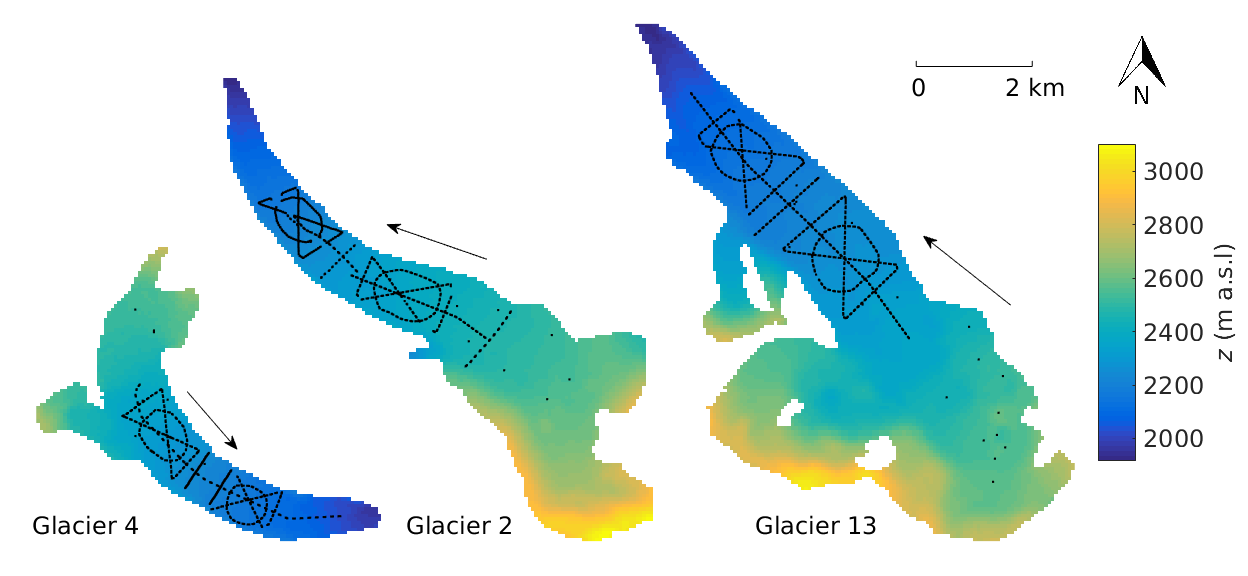
\includegraphics[height = 0.4\textwidth]{Map_elevation.png}\\
	\caption{Values of elevation used in the topographic regressions for three study glaciers. This DEM is derived from a SPOT5 satellite image and has a grid size of 40x40 m. Subsequent topographic parameters were derived from this DEM.}
	\label{map:elev}
\end{figure}

\begin{figure}
	\centering
	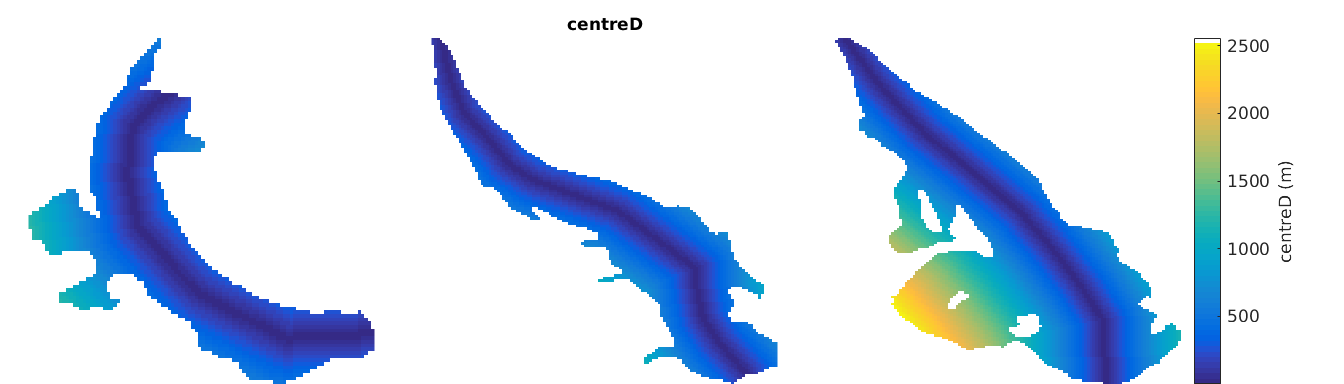
\includegraphics[height = 0.4\textwidth]{Map_centreD.png}\\
	\caption{Values of distance from centreline used in the topographic regressions for three study glaciers. Centreline was drawn by hand in QGIS.}
	\label{map:centreD}
\end{figure}

\begin{figure}
	\centering
	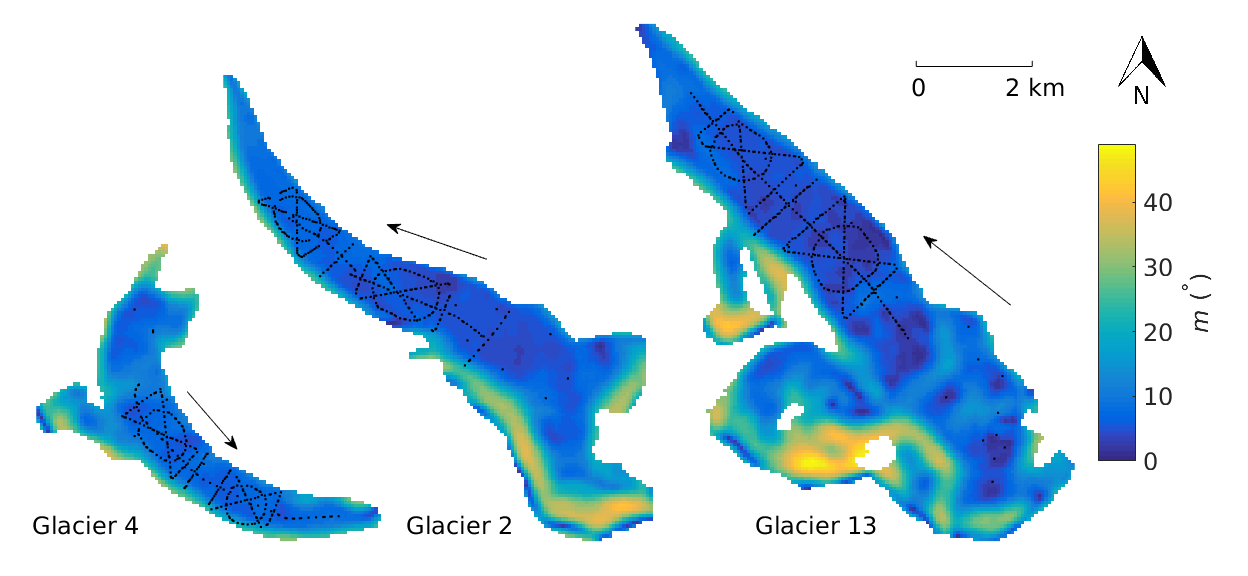
\includegraphics[height = 0.4\textwidth]{Map_slope.png}\\
	\caption{Values of slope used in the topographic regressions for three study glaciers. Values were derived from a SPOT5 satellite derived DEM (grid size of 40x40 m) in QGIS.}
	\label{map:slope}
\end{figure}

\begin{figure}
	\centering
	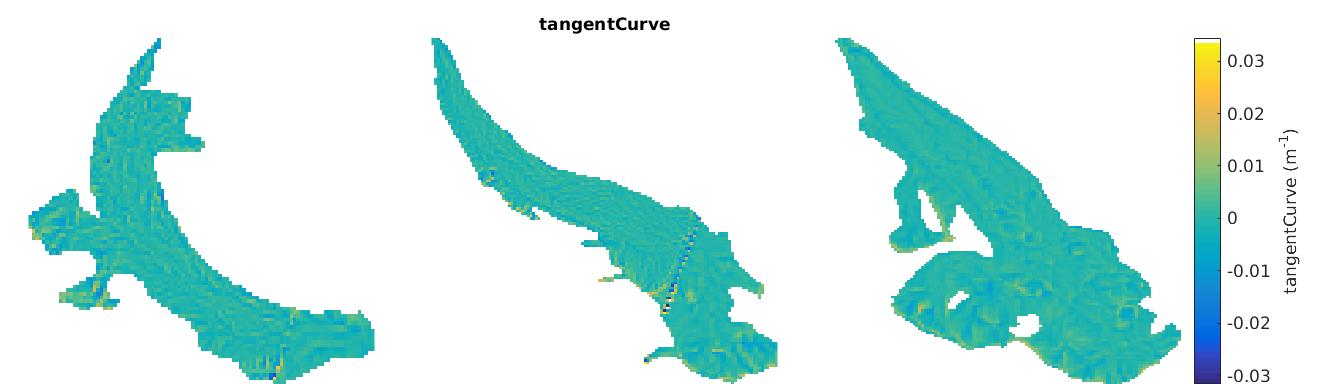
\includegraphics[height = 0.4\textwidth]{Map_tangentCurve.png}\\
	\caption{Values of tangential curvature used in the topographic regressions for three study glaciers. Values were derived from a SPOT5 satellite derived DEM (grid size of 40x40 m) in QGIS.}
	\label{map:tangentC}
\end{figure}

\begin{figure}
	\centering
	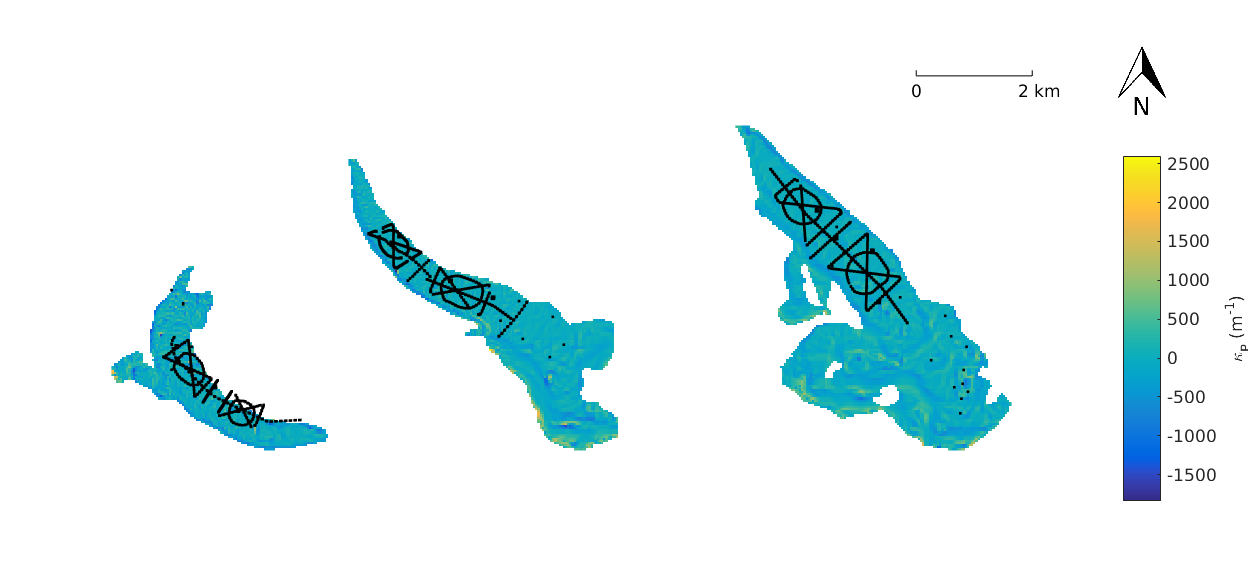
\includegraphics[height = 0.36\textwidth]{Map_profileCurve.png}\\
	\caption{Values of distance from centreline used in the topographic regressions for three study glaciers. Values were derived from a SPOT5 satellite derived DEM (grid size of 40x40 m) in QGIS.}
	\label{map:profileC}
\end{figure}

\begin{figure}
	\centering
	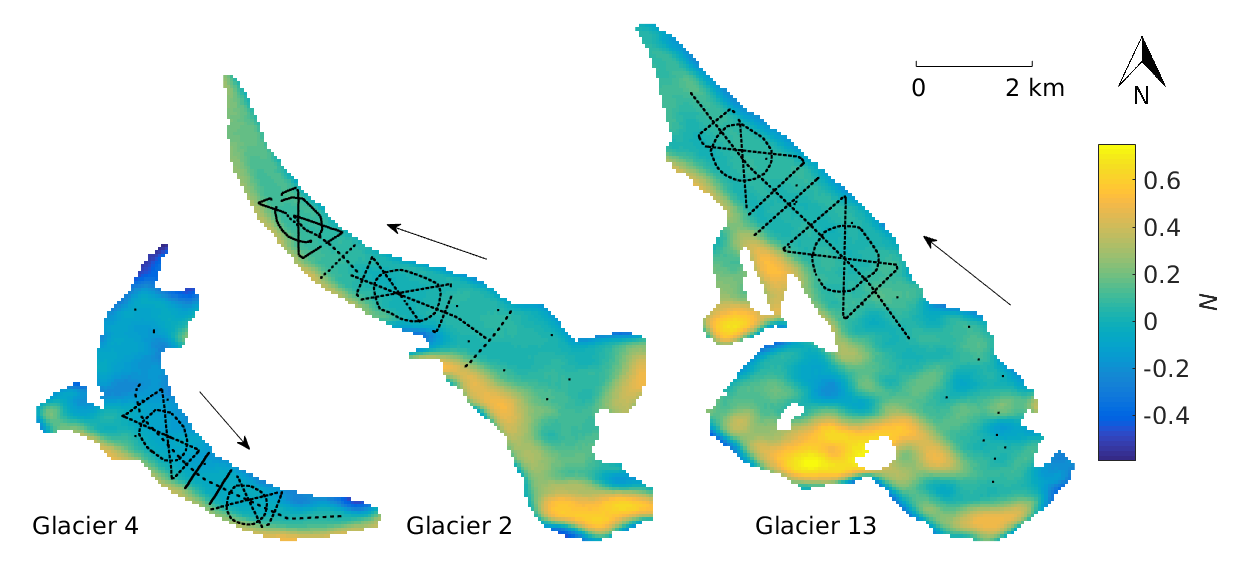
\includegraphics[height = 0.36\textwidth]{Map_northness.png}\\
	\caption{Values of ``northness'' used in the topographic regressions for three study glaciers. ``Northness'' is defined as the product of the cosine of aspect and sine of slope. A value of -1 represents a steep, south facing slope, a value of +1 represents a steep, north facing slope, and flat surfaces yield 0. Values were derived from a SPOT5 satellite derived DEM (grid size of 40x40 m) in QGIS.}
	\label{map:northness}
\end{figure}

\begin{figure}
	\centering
	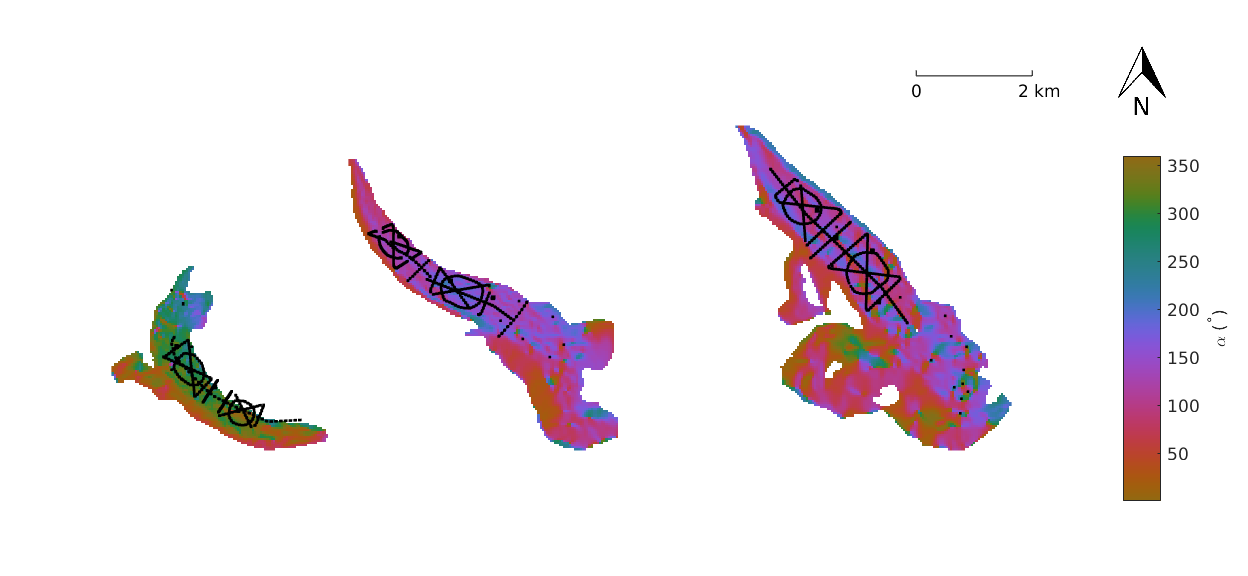
\includegraphics[height = 0.4\textwidth]{Map_aspect.png}\\
	\caption{Values of aspect, which represent what direction a slope is facing (0${^\circ}$ defined as north), used in the topographic regressions for three study glaciers.}
	\label{map:aspect}
\end{figure}

\begin{figure}
	\centering
	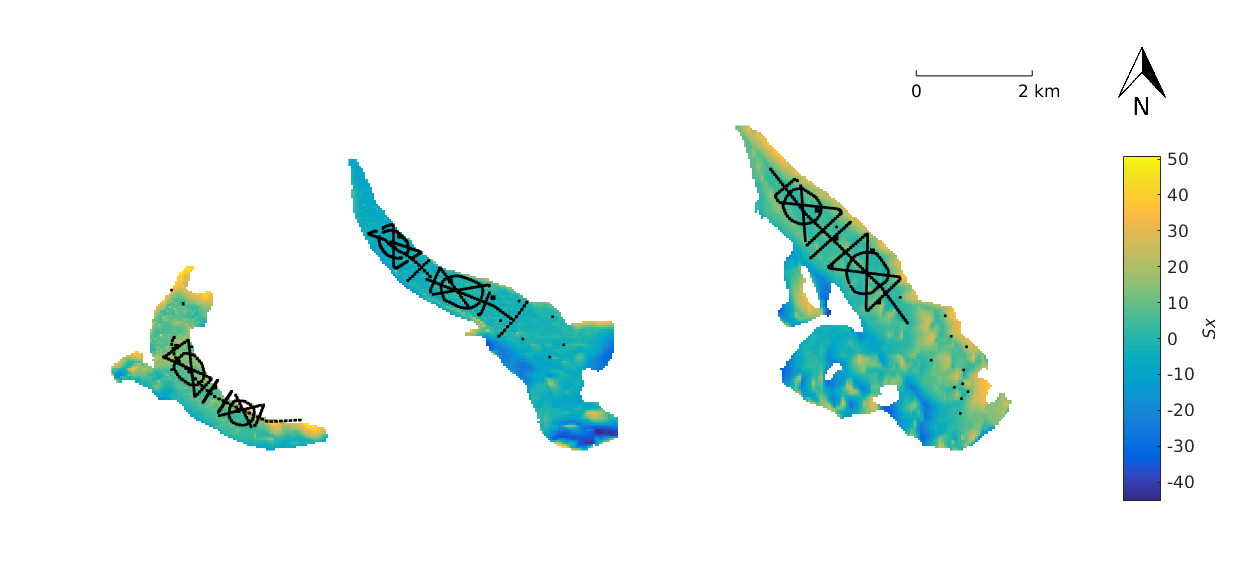
\includegraphics[height = 0.4\textwidth]{Map_Sx.png}\\
	\caption{Values of $Sx$, which is a wind redistribution parameter, used in the topographic regressions for three study glaciers. See section \ref{Sec:Sx} and the original paper by \cite{Winstral2002} for more details on calculation .}
	\label{map:Sx}
\end{figure}

\end{landscape}

\subsection{Range of parameters sampled}

\begin{landscape}

\begin{figure}
	\centering
	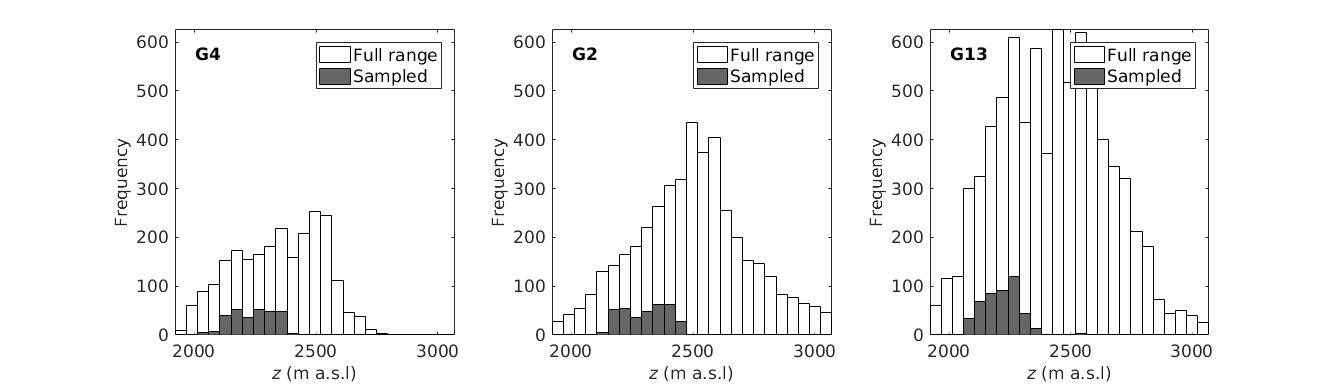
\includegraphics[height = 0.4\textwidth]{SampledRangeTopo_elevation.png}\\
	\caption{Range of elevation sampled as compared to total range of elevation of study glaciers.}
	\label{sampledRange:elev}
\end{figure}

\begin{figure}
	\centering
	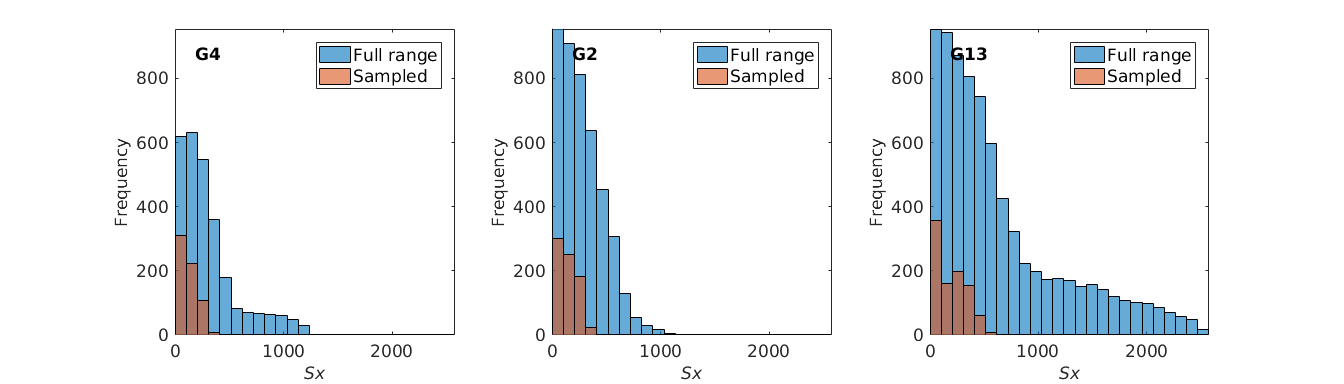
\includegraphics[height = 0.4\textwidth]{SampledRangeTopo_centreD.png}\\
	\caption{Range of distance from centreline sampled as compared to total range of distance from centreline of study glaciers.}
	\label{sampledRange:centreD}
\end{figure}

\begin{figure}
	\centering
	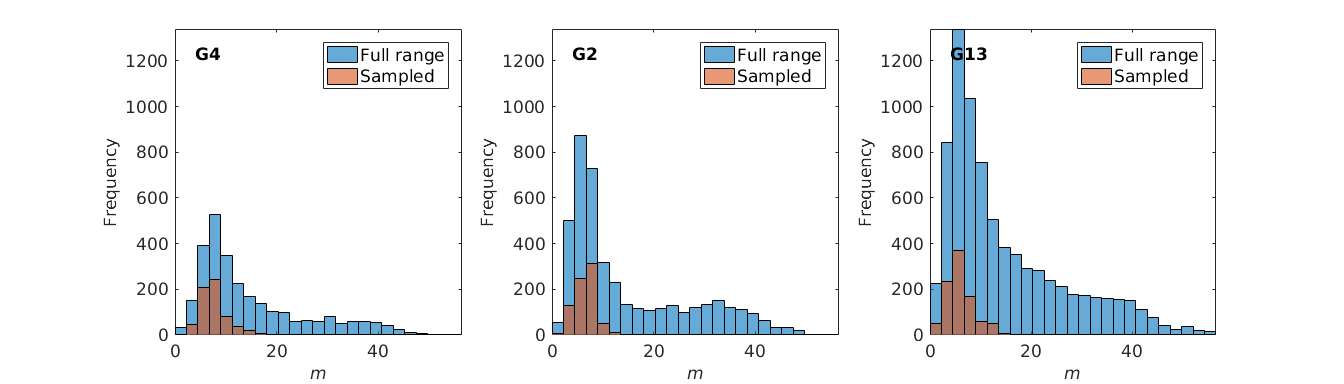
\includegraphics[height = 0.4\textwidth]{SampledRangeTopo_slope.png}\\
	\caption{Range of slope sampled as compared to total range of slope of study glaciers.}
	\label{sampledRange:slope}
\end{figure}

\begin{figure}
	\centering
	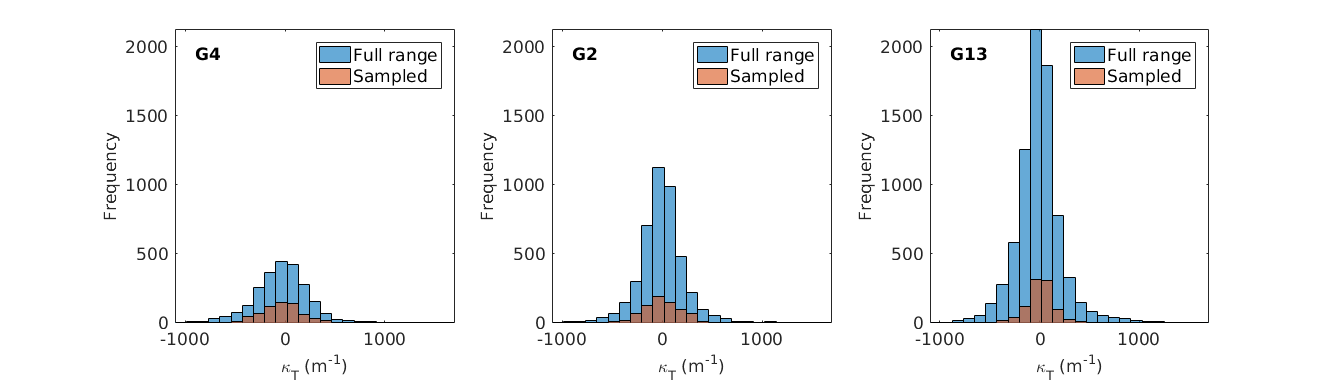
\includegraphics[height = 0.4\textwidth]{SampledRangeTopo_tangentCurve.png}\\
	\caption{Range of tangential curvature sampled as compared to total range of tangential curvature of study glaciers.}
	\label{sampledRange:tangentC}
\end{figure}

\begin{figure}
	\centering
	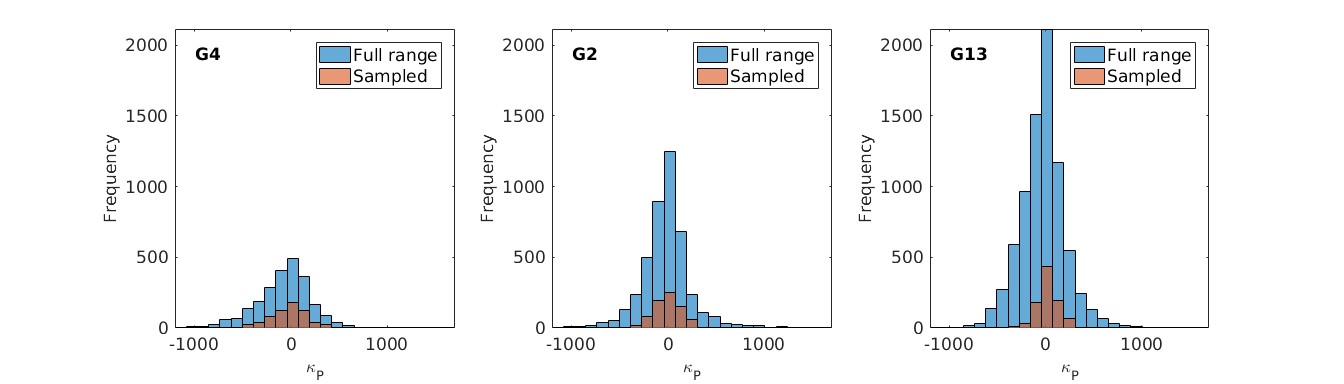
\includegraphics[height = 0.4\textwidth]{SampledRangeTopo_profileCurve.png}\\
	\caption{Range of profile curvature sampled as compared to total range of profile curvature of study glaciers.}
	\label{sampledRange:profileC}
\end{figure}

\begin{figure}
	\centering
	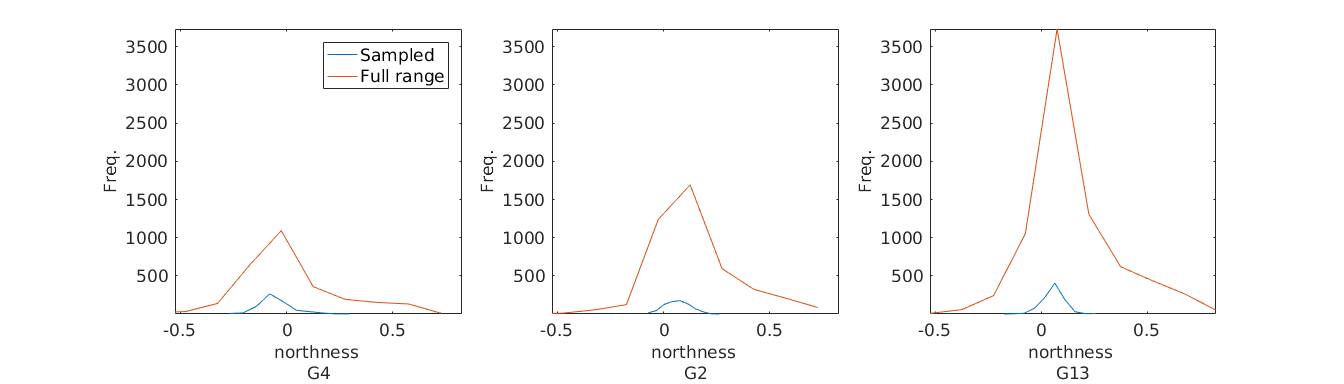
\includegraphics[height = 0.4\textwidth]{SampledRangeTopo_northness.png}\\
	\caption{Range of ``northness'' sampled as compared to total range of ``northness'' of study glaciers.}
	\label{sampledRange:northness}
\end{figure}

\begin{figure}
	\centering
	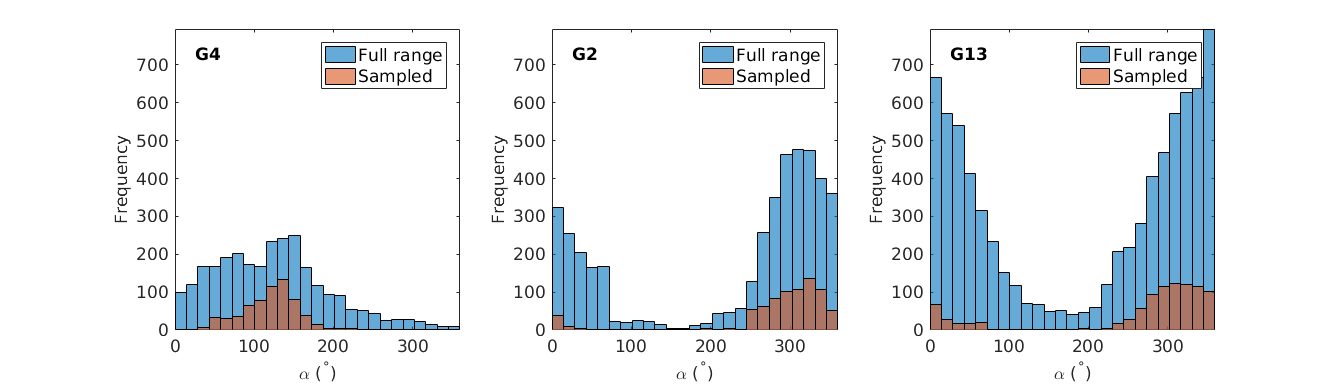
\includegraphics[height = 0.4\textwidth]{SampledRangeTopo_aspect.png}\\
	\caption{Range of aspect sampled as compared to total range of aspect of study glaciers.}
	\label{sampledRange:aspect}
\end{figure}

\begin{figure}
	\centering
	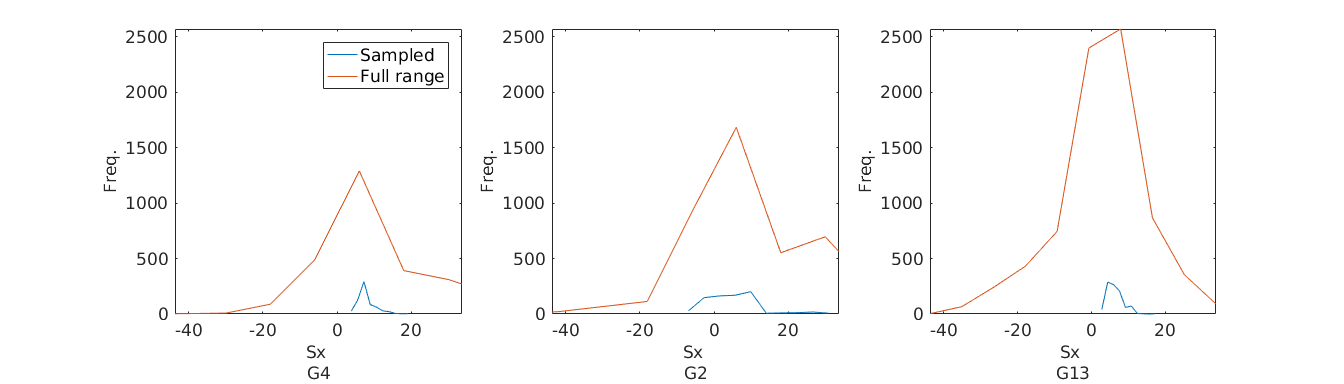
\includegraphics[height = 0.4\textwidth]{SampledRangeTopo_Sx.png}\\
	\caption{Range of $Sx$ sampled as compared to total range of $Sx$ of study glaciers.}
	\label{sampledRange:Sx}
\end{figure}

\end{landscape}


\section{Multiple Linear Regression}








 \begin{figure}
    \centering
    \begin{subfigure}[b]{0.38\textwidth}
        \fbox{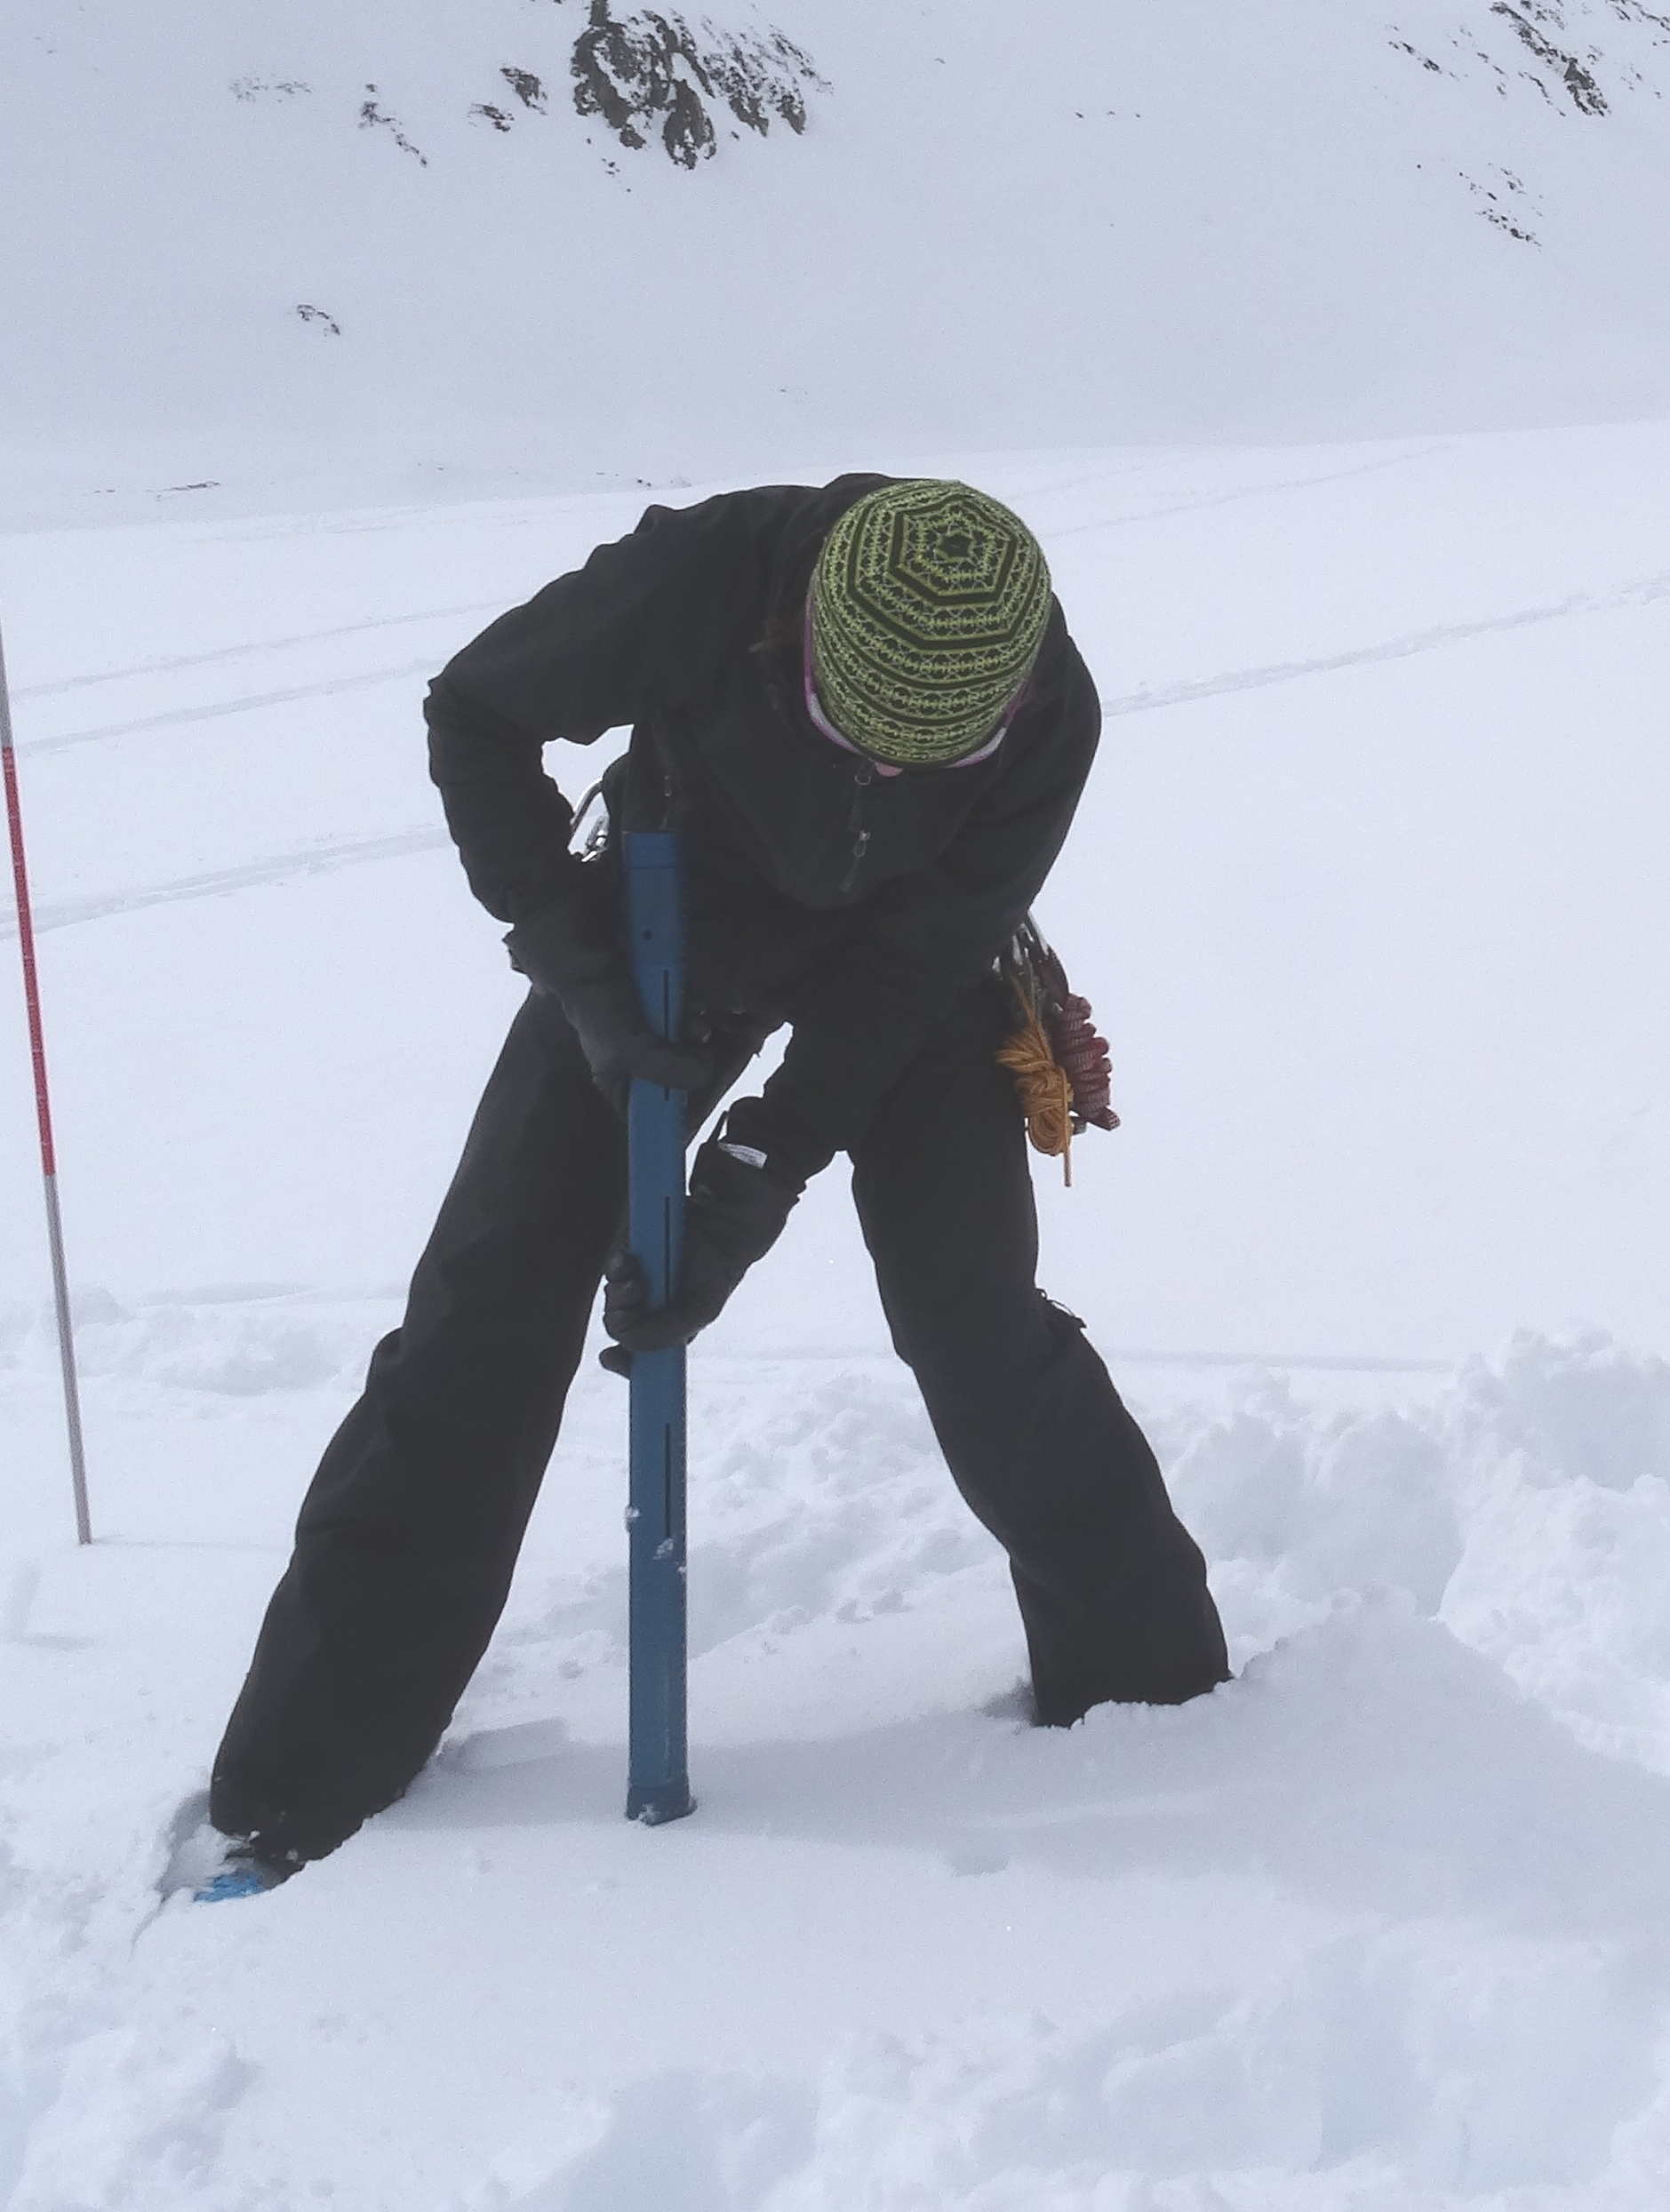
\includegraphics[width=\textwidth]{photo_swe1.JPG}}
        \caption{Inserting the Federal Sampler into the snow. Photo credit: C. Ariagno}
        \label{photo_swe1}
    \end{subfigure}
    ~
    \begin{subfigure}[b]{0.56\textwidth}
        \fbox{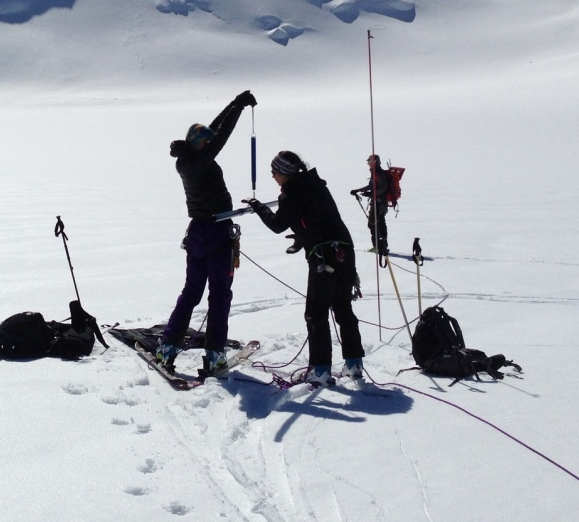
\includegraphics[width=\textwidth]{photo_swe2.jpg}}
        \caption{Weighing the Federal Sampler with snow core on the spring scale (units of cm SWE). Photo credit: G. Flowers}
        \label{photo_swe2}
    \end{subfigure}

    \caption{Using the Federal Sampler to measure SWE}
    \label{photo_swe}
\end{figure}
 
	
%%%%%%%%

\bibliography{/home/glaciology1/Documents/MastersDocuments/MastersLit}
\bibliographystyle{igs}

\end{document}